\section{Survival of small populations}
\label{sec:small}

Return to the binary Galton--Watson process near criticality, with \(p\) and \(1-p\) each close to one half. A lineage dies at the first generation with probability about \(\tfrac12\). Conditional on dividing, both daughters fail at their first attempt with probability about \(\tfrac14\), so the chance of still being alive at generation two is only about \(0.375\):
\begin{equation*}
0.375 \approx \underbrace{(1-0.5)}_{\text{survive step 1}}\times\underbrace{(1-0.5\times0.5)}_{\text{survive step 2}} .
\end{equation*}
Iterating the \pgf{} gives the precise early values. With \(\phi(z)=pz^2+(1-p)\),
\begin{equation}
\label{ext}
u_{n+1} = p\,u_n^2 + 1-p ,
\qquad
S_{n+1} = 2pS_n - pS_n^2 ,
\end{equation}
started at \(u_0=0\), \(S_0=1\). At exact criticality the first four extinction probabilities are
\begin{equation*}
u_n = 0.500,\ 0.625,\ 0.695,\ 0.741\quad(3\ \text{s.f.}),
\end{equation*}
so survival decays quickly even just above criticality (\cref{fig:earlySn}).

\begin{figure}[ht]
\centering
  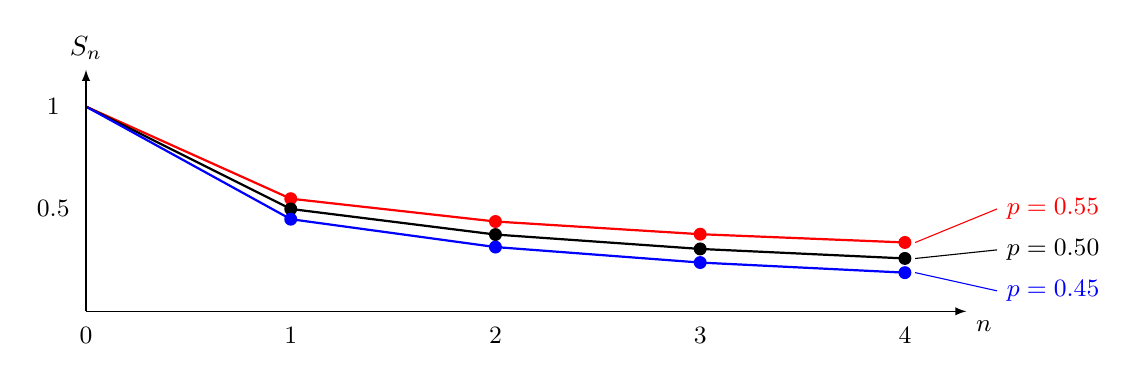
\begin{tikzpicture}[scale = 2.6]
    \foreach \x/\y/\color in {1/0.55/red, 2/0.4386250/red, 3/0.3766719/red, 4/0.336304/red,
                              1/0.5/black, 2/0.375/black, 3/0.3046875/black, 4/0.25827/black,
                              1/0.449999/blue, 2/0.313874/blue, 3/0.2381546/blue, 4/0.188816/blue}
      \fill[color=\color] (\x, \y) circle (0.9pt);
    \draw[red, thick] (0, 1) -- (1, 0.55) -- (2, 0.4386250) -- (3,0.3766719) -- (4,0.336304);
    \draw[black, thick] (0, 1)--(1,0.5) --  (2,0.375) -- (3,0.304687) -- (4,0.25827);
    \draw[blue, thick] (0, 1)--(1,0.449999)  --  (2,0.313874) -- (3,0.238154) -- (4,0.18881);
    \draw[-latex] (0,0) -- (4.3,0) node[below right, font=\small] {$n$};
    \draw[-latex] (0,0) -- (0,1.18) node[above] {$S_n$};
    \foreach \x/\lab in {0/0, 1/1, 2/2, 3/3, 4/4} \node[font=\small] at (\x, -0.12) {\lab};
    \foreach \y/\lab in {0.5/0.5, 1/1} \node[font=\small] at (-0.16, \y) {\lab};
    \draw[red,  thin] (4.05,0.336) -- (4.45,0.50);
    \draw[black,thin] (4.05,0.258) -- (4.45,0.30);
    \draw[blue, thin] (4.05,0.189) -- (4.45,0.10);
    \node[red,  font=\small, anchor=west] at (4.45, 0.50) {$p=0.55$};
    \node[black,font=\small, anchor=west] at (4.45, 0.30) {$p=0.50$};
    \node[blue, font=\small, anchor=west] at (4.45, 0.10) {$p=0.45$};
  \end{tikzpicture}
\caption{Survival probability over the first four generations from a single progenitor, from \cref{ext}. Even for \(p=0.55\) the early decay is steep; the three curves have barely separated by \(n=4\).}
\label{fig:earlySn}
\end{figure}

\subsection{An initial cohort of size \texorpdfstring{$k$}{k}}
\label{sec:cohort}

Now take \(\zz_0=k\): the process begins with a small founding group (for instance \(k=10\) pathogenic particles). Under supercritical growth the law of large numbers eventually stabilises the trajectory, but the founding phase is precisely where stochasticity dominates. The probability that at least one of the \(k\) independent lineages remains alive at generation \(n\) is
\begin{equation}
\label{eq:Snk}
S^{(k)}_n = 1 - \bigl({}_1u_n\bigr)^{k},
\end{equation}
where \({}_1u_n\) is the single-lineage extinction probability.

\begin{figure}[ht]
\centering
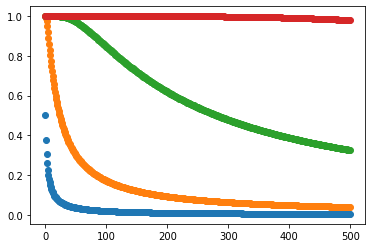
\includegraphics[width=0.56\textwidth]{figures/IMG_ch3/kvals.png}
\caption{Survival probability \(S^{(k)}_n\) from \cref{eq:Snk} out to \(500\) generations at exact criticality, \(p=0.5\), for \(k=1,10,100,1000\) (blue through to red). A larger founding cohort buys longevity, but at criticality every curve still tends to zero.}
\label{fig1}
\end{figure}

\begin{figure}[ht]
\centering
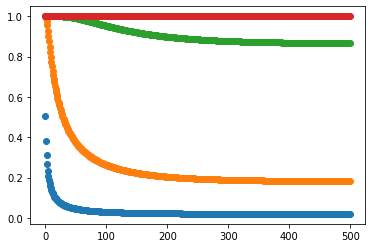
\includegraphics[width=0.45\textwidth]{figures/IMG_ch3/kvals505.png}
\hfill
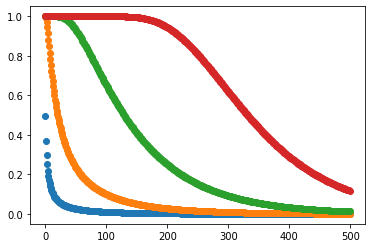
\includegraphics[width=0.45\textwidth]{figures/IMG_ch3/kvals495.png}
\caption{As \cref{fig1}, with \(p\) displaced slightly from criticality: \(p=0.505\) (left, supercritical) and \(p=0.495\) (right, subcritical). A half-percent shift separates curves that were nearly coincident at criticality.}
\label{fig2}
\end{figure}

\Cref{fig1,fig2} show \(S_n^{(k)}\) through \(500\) generations. The benefit of a larger inoculum is acutely sensitive to which side of \(\tfrac12\) the process sits on.

\subsection{An aside on early replication}
\label{sec:earlyrep}

The same conditioning effect appears in a different setting: the longevity and diversity of phylogenetic clades. Clades that persist to the present tend to show elevated early origination rates in the fossil record. Budd and Mann \cite{Budd2018} argue that this need not reflect a biological slowdown later on: if one simulates many homogeneous birth--death processes and retains only those still alive at a large observation time, the retained set is automatically enriched for early rapid growth --- the \emph{push of the past}. That is the conditioning of \cref{sec:qsd} read the other way: there one conditions a subcritical process on survival and finds a finite quasi-stationary mean; here one conditions a critical or supercritical process on survival to the present and finds inflated early growth.

On the pathogenic side the parallel suggests that securing a high probability of early replication may matter disproportionately, even if later per-capita rates are less favourable. \Cref{fig:earlySn} makes the point quantitatively: the first few generations concentrate most of the extinction risk.

\subsection{Discrete birth--death--catastrophe}
\label{sec:bdc}

Until catastrophe fires, a discrete-time birth--death--catastrophe process behaves, for the purpose of limiting conditional laws given non-extinction and non-rupture, like the Galton--Watson model above. Whether a quasi-stationary distribution survives when one conditions only on avoiding both death and catastrophe is a separate question, best settled by simulation for a given rate structure. In any case the probability of avoiding catastrophe is needed as a building block. Full continuous-time birth--death--catastrophe analysis --- means, variances, burst sizes, and quasi-stationarity under rupture --- is developed in Chapters~3--5; here we record the discrete survival formulae from the seed material and define the continuous rates.

\subsubsection*{Probability of rupture at step \texorpdfstring{$n$}{n}}

Let \(\kappa\) be the probability that a given individual initiates catastrophe at a step. A cohort of size \(N\) fails to rupture with probability \((1-\kappa)^N\).

In the birth-and-catastrophe case with no death, the living census is deterministic: from a single progenitor the population doubles at each step prior to catastrophe. Rupture occurs at generation \(n\) with probability
\begin{equation*}
1-(1-\kappa)^{2^{\,n-1}},
\end{equation*}
one minus the probability that none of the \(2^{n-1}\) individuals present triggered it.

\subsubsection*{Probability of process survival}

Still without death, let \(S_n\) be the probability that the process reaches generation \(n\) without catastrophe. Then \(S_0=1\), \(S_1=1-\kappa\), and survival to step \(2\) requires the founder and both offspring to avoid rupture:
\begin{equation*}
S_2 = (1-\kappa)(1-\kappa)^2 .
\end{equation*}
In general
\begin{equation}
\label{eq:bdcS}
S_n = \prod_{i=0}^{n-1}(1-\kappa)^{2^i} = (1-\kappa)^{2^n-1}.
\end{equation}

\subsubsection*{Death included}

Once death is allowed, the living census is random. Replacing the random count by its mean in the survival product,
\begin{equation}
\label{eq:bdcguess}
S_n \overset{?}{=} (1-\kappa)^{\sum_{i=0}^{n-1}\mean{\xx_i}} ,
\end{equation}
is not an identity. The map \(N\mapsto(1-\kappa)^N\) is convex, so Jensen's inequality gives \(\mean{(1-\kappa)^{\xx_i}}\ge(1-\kappa)^{\mean{\xx_i}}\): the mean underestimates the chance of passing a step. Surviving one step is also informative about a smaller population, which raises the chance of surviving the next. Both effects act in the same direction, so \cref{eq:bdcguess} is better read as a lower bound than as an equality.

\subsubsection*{Continuous-time BDC (definition and forward pointer)}

In continuous time, a single-type birth--death--catastrophe process on \(\{0,1,2,\dots\}\) with per-capita birth rate \(\lambda\), death rate \(\mu\), and catastrophe rate \(\delta\) has transitions
\begin{equation}
\label{eq:bdc-ct-rates}
i \to i+1 \text{ at rate } i\lambda,\qquad
i \to i-1 \text{ at rate } i\mu,\qquad
i \to R \text{ at rate } i\delta,
\end{equation}
where \(R\) is an absorbing rupture state. The process encodes intracellular load growth with load-dependent risk of host-cell rupture. Means, generating-function PDEs, burst-size distributions, and quasi-stationary structure for this model (and its two-type extensions) are developed in Chapters~3--5; the present chapter supplies the branching, quasi-stationary, and characteristics tools those chapters use.

\subsection{Continuous-time birth--death}
\label{sec:cts}

The discrete constant \(A(p)\) has no elementary closed form (\cref{sec:Ap}). Its continuous-time counterpart does, and the comparison is informative.

For the linear birth--death process with per-capita rates \(\lambda\) and \(\mu\), started from \(N\) individuals, the extinction probability is \cite{Allen2010}
\begin{equation}
\label{eq:p0t}
p_0(t) = \begin{cases}
\lrb{\dfrac{\mu - \mu \ee^{(\mu-\lambda)t}}{\lambda - \mu \ee^{(\mu-\lambda)t}}}^{N}, & \lambda \neq \mu,\\[12pt]
\lrb{\dfrac{\lambda t}{1+\lambda t}}^{N}, & \lambda = \mu,
\end{cases}
\end{equation}
and \(S^{(N)}(t)=1-p_0(t)\).

\subsubsection*{Limiting mean conditioned on non-extinction}

When \(\mu>\lambda\) (subcritical), the conditional mean settles. With \(N=1\),
\begin{equation*}
\mean{\xt}=\ee^{(\lambda-\mu)t},
\qquad
S(t)=\frac{\lambda-\mu}{\lambda - \mu\ee^{(\mu-\lambda)t}},
\end{equation*}
so
\begin{equation*}
\mean{\xt \mid \xt > 0} = \frac{\lambda\ee^{(\lambda-\mu)t} - \mu}{\lambda-\mu}
\xrightarrow{t\to\infty}
\frac{\mu}{\mu-\lambda}.
\end{equation*}
Writing \(p=\lambda/(\lambda+\mu)\) so that \(\lambda/\mu=p/(1-p)\),
\begin{equation}
\label{eq:Acts}
A_{\text{c}}(p) = \frac{1-2p}{1-p},
\qquad
\frac{1}{A_{\text{c}}} = \frac{1-p}{1-2p}.
\end{equation}
The subscript marks the continuous-time constant, distinguished from the discrete \(A(p)\) of \cref{lateS}.

\begin{figure}[ht]
\centering
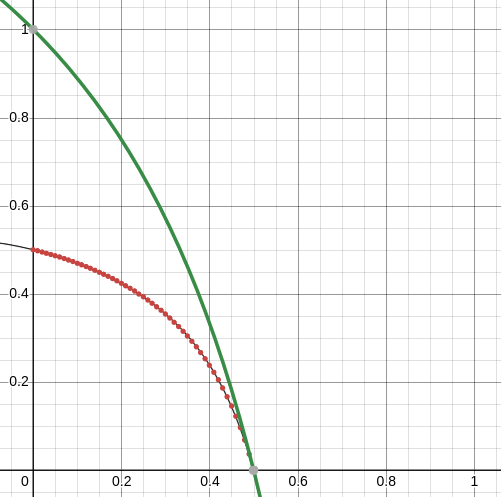
\includegraphics[width=0.5\textwidth]{figures/IMG_ch3/dtctA.png}
\caption{Continuous-time \(A_{\text{c}}(p)=(1-2p)/(1-p)\) (green) against high-precision numerical values of discrete \(A(p)\) (red). Both vanish at \(p=\tfrac12\), but at \(p=0\) the continuous curve starts at \(1\) and the discrete one at \(\tfrac12\); they are not related by a constant factor. The black curve is a symbolic-regression candidate from \cref{sec:GA}; it tracks the points closely but is not exact. \Cref{sec:compare} accounts for the discrepancy.}
\label{fig:dtct}
\end{figure}

\Cref{fig:dtct} raises the natural question: why do the curves start at different heights yet meet near criticality? \Cref{sec:compare} answers once the series representation of \(A(p)\) is available.

\FloatBarrier
